




\chapter{Validation of Injection Channel}

Without loss of generality, We injected binary blackhole signals to test performance of our De-Whitening Filter. Unfortunately we couldn't find a compatible data-taking system with desired noise level and dynamical range to reconstruct or estimate the expect End-Test Mirror (ETM) that generated by our Photon Calibrator. 

  

\begin{figure}[hbt!]
\centering
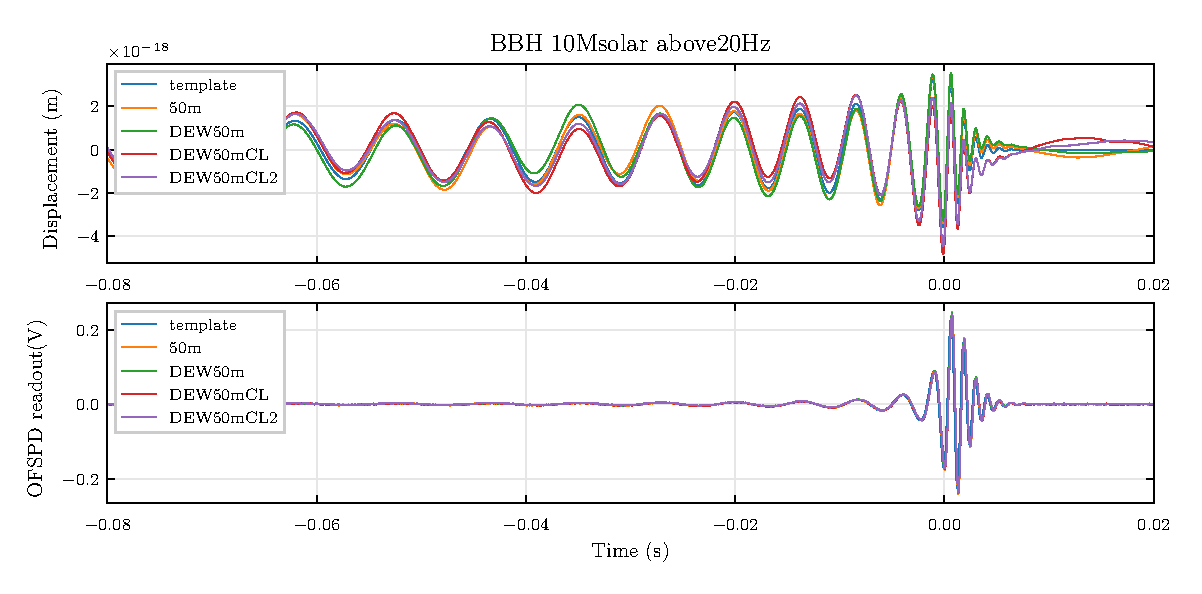
\includegraphics[width=\textwidth]{figure/inj/10.eps}


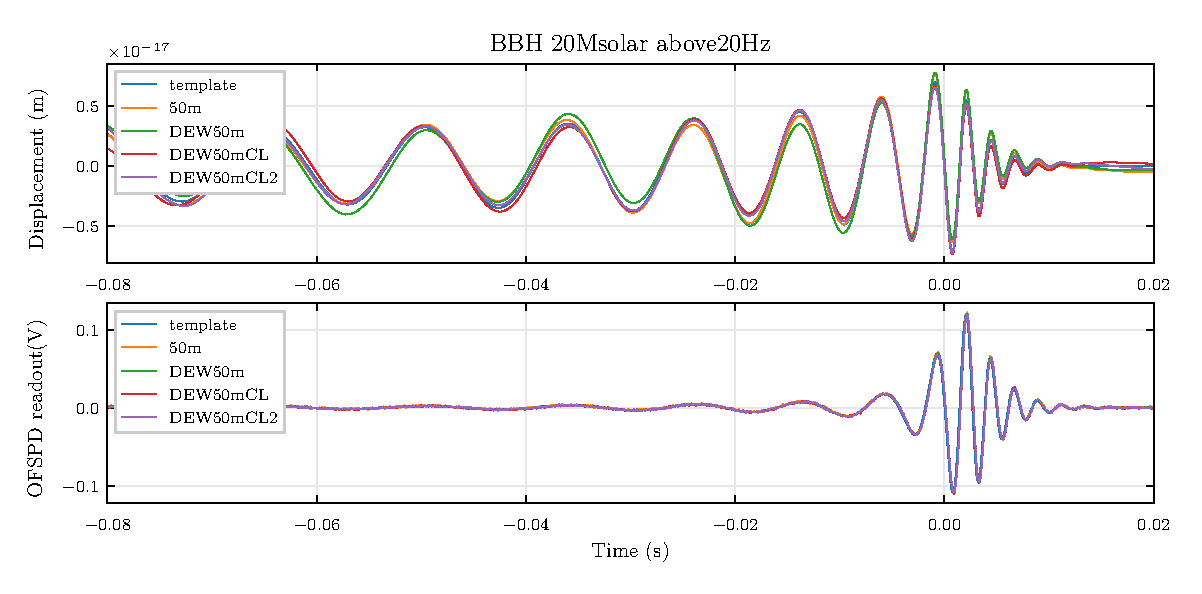
\includegraphics[width=\textwidth]{figure/inj/20.eps}


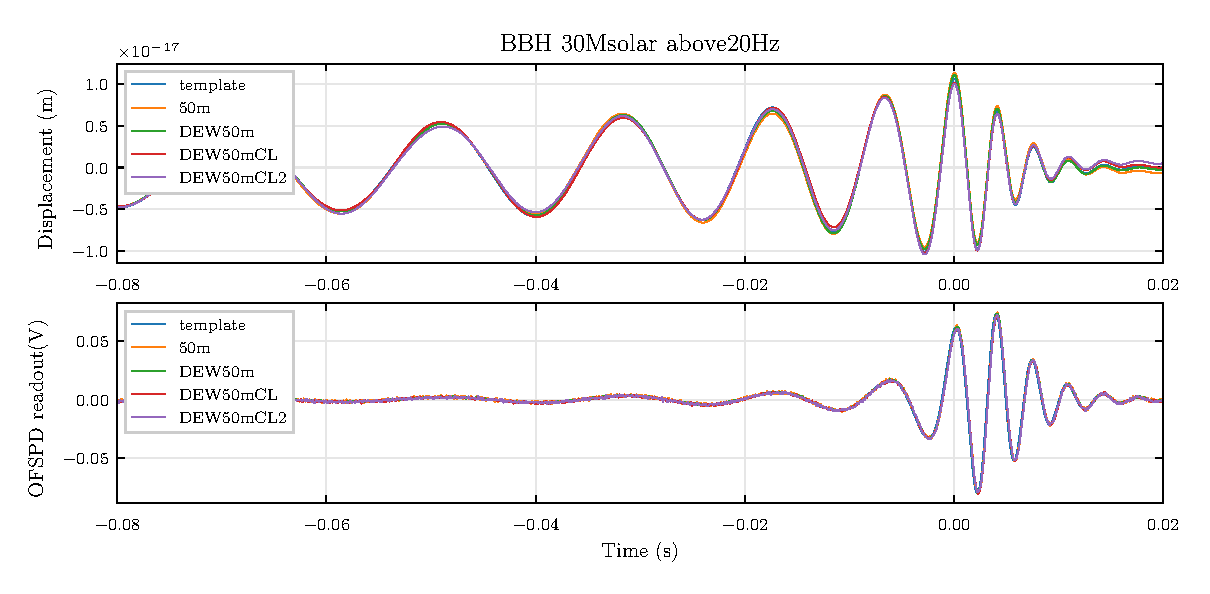
\includegraphics[width=\textwidth]{figure/inj/30.eps}
\caption{Injected Binary Blackhole Merger Signal}\label{fig:bbhinj}
\index{figures}
\end{figure}


Besides, We have tried to inject Sine-Gaussian signals.




Noise measurement
around 100Hz  the nose should below the IFO sensitivity
Transfer Function measurement
“above 1kHz” performance
time delay of excitation channel
(absolute timing measurement?)
Distortion of Scientific Signal
BBH
BNS post merger



